\documentclass[10pt,a4paper]{article}
\usepackage[latin1]{inputenc}
\usepackage{amsmath}
\usepackage{amsfonts}
\usepackage{amssymb}
\usepackage{graphicx}
\usepackage{amssymb}
\author{Paul Wieland}
\title{INF3490 Mandatory Assignment 2:
	Multilayer Perceptron}
\date{Deadline: Tuesday, October 16th, 2018 23:59:00}
\begin{document}
	\maketitle
	\tableofcontents
	\newpage
	%%%%%%%%%%%%%%%%%%%%%%%%%%%%%%%%%%%%%%%%%%%%%%%% 	%INTRODUCTION
	\section{Introduction}
	\subsection{Task}									%task
	We will build a Multilayer Perceptron to steer a robotic prosthetic hand. There are 40 inputs of electromyographic signals that we will classify. \\
	There are 8 classification values corresponding to a different hand motion: \\
	\begin{center}
		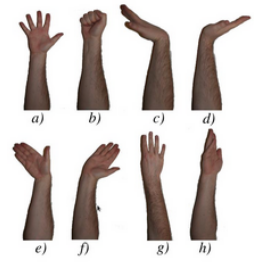
\includegraphics[width=0.4\linewidth]{pictures/hand}
		\\
		Figure 1: Possible motions \footnote{http://folk.uio.no/kyrrehg/pf/papers/glette-ahs08.pdf}
		\\
	\end{center}
	\begin{center}
		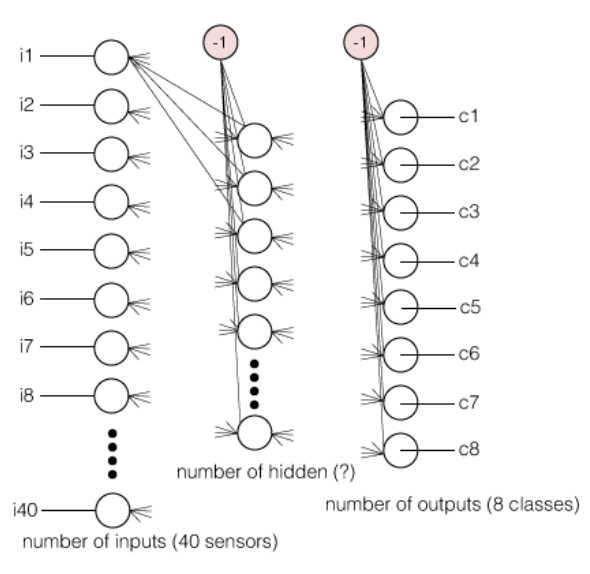
\includegraphics[width=0.7\linewidth]{pictures/mlp}
		\\
		Figure 2: Multilayer Perceptron for our problem \footnote{https://www.uio.no/studier/emner/matnat/ifi/INF3490/h18/assignments/assignment-2/assignment\_2.pdf}
		\\
	\end{center}
	We build a Multilayer Perceptron with 40 entry nodes, that means one node for each input. Then, there is one hidden layer with a various number of hidden nodes. For classifying the input, there are 8 output nodes corresponding to the 8 hand motions. We only use one hidden layer to solve this problem.

	\subsection{Training Data}							%training data
	For each input vector:
	\begin{center}

		\begin{equation}
		input = [i_1,i_2,i_3,i_4,...,i_{40}], i_n \in  \mathbb{R},n \in [40]
		\end{equation}
	\end{center}
	we have a target output vector:
	\begin{center}
		\begin{equation}
		 output = [c_1,c_2,c_3,c_4,...,c_8], c_n \in \{0,1\}, n \in [8],\sum_{n=1}^{8} c_n  = 1 
		 \end{equation}  
	\end{center}
	That means, forwarding the input should result in the given target vector. 
	%%%%%%%%%%%%%%%%%%%%%%%%%%%%%%%%%%%%%%%%%%%%%%%%		%IMPLEMENTATION
	\section{Implementation}
	The file \textit{mlp.py} contains the class mlp. In \textit{operations.py} are implemented some general functions to test them easily.
	To run the Multilayer Perceptron just execute the file(python3):
	\begin{center}
			\textit{python3 movements.py}
	\end{center}
	\subsection{Initialization}								%initalization
	The function \textit{ \_\_init\_\_(self, inputs, targets, nhidden)} has three important parameter that we need to initialize the Multilayer Perceptron. \\
	As the input data is given as a vector, it is a good choice to create two 2D-Array for the two weight layers. As the parameters \textit{inputs} and \textit{targets} have the type \textit{$<$class 'numpy.ndarray'$>$}, it is a good idea to work only with numpy arrays. \\
	\subsubsection{Dimension of the weight matrix}			%Dimension of weight matrix
		\begin{itemize}
		\item weight\_matrix\_1: \\
		The input vector in (1) has of course a size of 40. But we need to add the \textit{bias\_value -1} that can be seen in Figure 2. That means: \\ 
		\begin{center}
			\begin{equation}
			 \textit{weight\_matrix\_1} \in \mathbb{R}^{41 \times nhidden} 
			\end{equation} 
			\\
			 $w_{i,j} \in weight\_matrix\_1, w_{i,j}$: weight between input/bias node(i) and hidden node(j) 
		\end{center}
		\item weight\_matrix\_2: \\
		There are \textit{nhidden} hidden nodes and 8 exit nodes. So we also need to take into account the \textit{bias\_value -1}. That means: \\
		\begin{center}
			\begin{equation}
			\textit{weight\_matrix\_2} \in \mathbb{R}^{(nhidden+1) \times 8} 
			\end{equation}
			\\
			$w_{i,j} \in weight\_matrix\_1, w_{i,j}$: weight between hidden/bias node(i) and output node(j)  
		\end{center}
	\end{itemize} 
	Both, \textit{weigh\_matrix\_1} and \textit{weigh\_matrix\_2}, will be initialized randomly with values in [-1,1].
	
	\subsection{Forward}								%forward
	The forward function takes one input vector and runs it on the network. At first, the input vector must be expanded by -1. The reason for this is that we have to take into account the bias value:	
	\begin{center}
		\begin{equation}
		\textit{input} \in \mathbb{R}^{1\times 41} 
		\end{equation} 
	\end{center}
	\subsubsection{Forward Phase 1}
	Subsequently it is possible to compute the \textit{hidden\_values}:
	\begin{center}
		\begin{equation}
		\textit{hidden\_values} = [h_1,h_2,h_3,h_4,...,h_8]
		\end{equation} 
	\end{center}

	\begin{center}
		\begin{equation}
		h_i = \sum_{n=1}^{41} input[n] \times weight\_matrix\_1[n][i] 
		\end{equation} 
	\end{center}
	This operation is done by the function \textit{ vec\_matr\_mult()} (that function can be found in the file \textit{operations.py}) that is doing a vector matrix multiplication with two for-loops. \\
	\subsubsection{Activation Function}
	After that is the activation function applied to all hidden nodes, as well to the bias node:
	\begin{center}
		\begin{equation}
		a_{\zeta} = h_{new, i} = \frac{1}{1 + \ exp(-\beta h_i)} 
		\end{equation} 
		\\ (\textit{apply\_sigmoid\_activation()} in \textit{operations.py})
	\end{center}
	\subsubsection{Forward Phase 2}
	The result \textit{hidden\_values} is therefor: 
	\begin{center}
		\begin{equation}
		\textit{hidden\_activation} \in \mathbb{R}^{1\times (nhidden +1)} 
		\end{equation} 
	\end{center}
	 So the \textit{output} vector can be calculated easily by another vector matrix multiplication:
	  \begin{center}
	  	\begin{equation}
	  	\textit{output} = hidden\_activation \cdot weight\_matrix\_2 
	  	\end{equation} 
	  \end{center}
  	\subsubsection{Output Error}
  	For the first implementation a linear output function was used. But the behavior of the algorithm was not really good. So I decided to apply the sigmoid function (8) to the output as well. The error function for the output node is therefor: \\
  	\begin{center}
  		\begin{equation}
  		\delta_o (\kappa) = (y_{\kappa}-t_{\kappa})y_{\kappa}(1-y_{\kappa})  
  		\end{equation} 
  	\end{center}
  	This works much better. For example, we can see that the target value converges to 1 and the other to 0. Here is an example of the training set: \\
  	\begin{center}
  			\begin{center}
  			\begin{tabular}{|l|c|c|c|c|c|c|c|c|}
  				\hline
  				output&	1.6e-02& 7.0e-02 & 1.6e-02 & 2.9e-02 & 4.7e-04 & 1.1e-05 & 6.6e-05& 8.4e-01\\ 
  				\hline
  				target&0&0  &0  &0  &0  &0  &0  &1 \\
  				\hline
  			\end{tabular}		
  		\end{center}
  	\end{center}
  	And another output of the validation set: \\
  	\begin{center}
  			\begin{tabular}{|l|c|c|c|c|c|c|c|c|}
  				\hline
  				output&1.6e-02& 1.0e-04 & 9.8e-01 & 9.4e-03 & 6.4e-05 & 2.6e-04 & 1.6e-02 & 2.0e-02\\ 
  				\hline
  				target&0&0  &1  &0  &0  &0  &0  &0 \\
  				\hline
  			\end{tabular}		
  	\end{center}
  	
  	\subsection{Calculate Hidden-Error}								%hidden error 
	From the forward phase we have gained the \textit{output-error}(11) and the \textit{activation-values}(7),(8) of the hidden nodes. That means it is possible to calculate the errors of the hidden nodes. The error of the hidden layer is determined by the function \textit{calculate\_hidden\_error()}. It follows the formula: \\
	 \begin{center}
		\begin{equation}
		\delta_h(\zeta) = a_{\zeta}(1-a_{\zeta}) \sum_{k=1}^{N} w_{\zeta}\delta_o(k) \quad, \beta =1
		\end{equation} 
	\end{center}
	Where:
	\begin{itemize}
		\item $ a_{\zeta} \in \textit{hidden\_activation} $, because $ \beta a_{\zeta}(1-a_{\zeta}) = \frac{d}{dh} \frac{1}{1 + \ exp(-\beta h_i)}$, see (8)
		\item $ w_{\zeta} \in \textit{weight\_matrix\_2}$, see (4)
		\item $ \delta_o(k) \ in \textit{output\_error} $, see (11)
	\end{itemize}
	So, $w_{\zeta}$ is the weight that connects a hidden node, with activation $a_{\zeta}$, and a output node with output-error $\delta_o(k)$.
	\subsection{Train the network}				%%%%%%%%%%%%%%%%%train the network
	To train the network means to backpropagate the errors we that we have calculated in 2.2.4 and 2.3. So the weights of \textit{weight\_matrix\_1} and \textit{weight\_matrix\_2} will be adjusted by the following formula:
	\begin{center}
		\begin{equation}
		w_{ij} = w_{ij} - \eta \delta_j x_i
		\end{equation} 
	\end{center}
	Where:
	\begin{itemize}
		\item $w_{ij}$ is the weight that connects an input node(i) and an output node(j). Input and output means only the activation direction, not any specific layer.
		\item $x_i$ is the activation value of an input node. From the view of \textit{weight\_matrix\_1} is the input vector of the network the meant input. From the view of \textit{weight\_matrix\_2} is the hidden layer the input one.
		\item  $\delta_j$ is the error of the output node.
		\item $\eta$ is the learning rate of the network. 

	\end{itemize}   
	\subsection{Earlystopping}				%%%%%%%%%%%%%%%%%earlystopping
	The function \textit{earlystopping()} observes the learning of the network. It should avoid overfitting. That means that the network is adjusted too much to the training data so unknown data will be classified very bad.
	\begin{center}
		\includegraphics[width=0.9\linewidth]{"pictures/Untitled Diagram"} \\
		Figure 1: Main flow of the Multilayer-Perceptron 
	\end{center}
	As you can see in the figure above, \textit{Sequential Training} is used. That means the network will be trained after one input vector. One iteration is therefor one iteration through the whole data input. That is also the reason why the input data will be randomized each iteration. The randomization should avoid learning the network with data in the same order. That may lead to bad generalization issues.
	\subsubsection{Decision earlystopping}		%%%%%%%%%%%%%%%%%decision earlystopping
	 As you can see in the graphic above, the algorithm trains the network for a certain number of iterations before the validation set will be applied.The validation set is unknown to the network. The Error-Function: \\
	 	\begin{center}
	 	\begin{equation}
	 	E(w) = \frac{1}{2} \sum_{k} (t_{\kappa} - y_{\kappa})^{2}
	 	\end{equation} 
	 \end{center}
 	is used to estimate the quality of the network. So after each epoch (one is a certain number of iterations, eg. 10,100,1000) the Error-Function will be applied to the validation set. If the error of one epoch if bigger than the epoch before, the algorithm stops to avoid overfitting.
 	\begin{center}
 		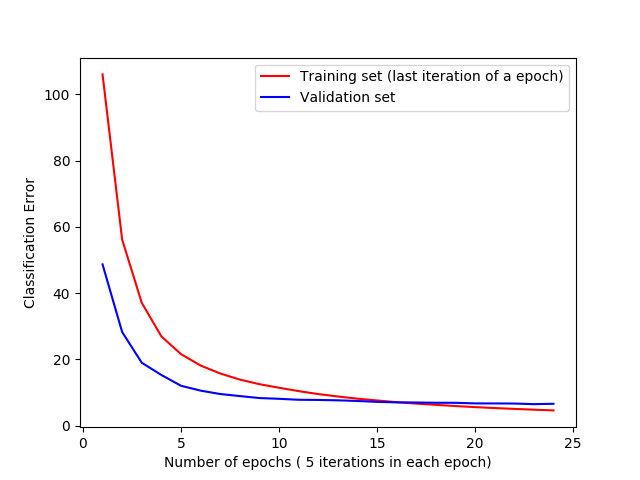
\includegraphics[width=0.8\linewidth]{pictures/earlystopping}
 		\\Figure 2: Effect of Earlystopping
 	\end{center}
 	In the graphic above you see very good how earlystopping works. Both, the Training-Error and the Validation-Error decrease. The Training-Error would reach zero if there is no stopping criteria. That means also that the Validation-Error would increase again because the network is not able to classify unknown data as good as when the algorithm stops earlier. So the Algorithm stops if the blue line starts to increase. 
 	\subsection{Confusion}					%%%%%%%%%%%%%%%%%confusion
 	For the confusion phase, a set of unknown data will be forwarded. The number of wrong classifications is represented as a confusion-matrix. Where on the x-axis are the target classes on on the y-axis the classifications that are made by the network.
 	
 	\section{Results}						%%%%%%%%%%%%%%%%RESULTS
 	The network will be tuned and forwarded to evaluate and compare the results. All tests are made with 10 iterations in each epoch. For each number of nodes were made 10 tests because the random initialization of the weight matrices can influence the quality of the result.
 	\\
 	I defined a correct class as a class that has no wrong classifications.
 	\subsection{Hidden Nodes: 6}
 	\begin{center}
 		$ confusion\_matrix = \begin{bmatrix}
 		12& 0& 0& 0& 1& 0& 0& 0  \\
 		0& 15& 0& 0& 0& 0& 0& 0 \\
 		0& 0& 13& 0& 0& 1& 0& 0 \\
 		0& 0& 0& 17& 0& 0& 0& 0 \\
 		2& 0& 0& 0& 11& 0& 0& 0 \\
 		1& 1& 0& 0& 0& 12& 0& 0 \\
 		0& 0& 0& 0& 0& 1& 10& 0 \\
 		0& 0& 0& 2& 0& 0& 0& 12 \\
 		\end{bmatrix}$
 	\end{center}
 	
 	\begin{tabular} {ll}
 		Percentage of correct classes: &  37.5 \% \\
 		Number of inputs: & 111 \\
 		Wrong classifications: & 9 \\
 		Percentage wrong classification: & 8.1 \% \\
 	\end{tabular}
 	\\ 
 	\\ \\
 	For more results see the file \textit{mlp\_6\_hidden\_nodes.txt}
 	
 	\subsection{Hidden Nodes: 12}
 		\begin{center}
 		$ confusion\_matrix = \begin{bmatrix}
 		11& 0& 0& 0& 1& 0& 0& 1 \\
 		0& 17& 0& 0& 0& 0& 0& 0 \\
 		0& 0& 14& 0& 0& 0& 0& 0 \\
 		0& 1& 0& 9& 0& 0& 0& 1 \\
 		0& 0& 0& 0& 16& 0& 0& 0 \\
 		0& 0& 0& 0& 0& 14& 0& 0 \\
 		0& 0& 0& 0& 0& 0& 13& 0 \\
 		0& 0& 0& 0& 0& 0& 0& 13 \\
 		\end{bmatrix}$
 	\end{center}
	 \begin{tabular} {ll}
	 	Percentage of correct classes: &  62.5 \% \\
	 	Number of inputs: & 111 \\
	 	Wrong classifications: & 4 \\
	 	Percentage wrong classification: & 3.6 \% \\
	 \end{tabular}
 	\\ 
 	\\ \\
 	For more results see the file \textit{mlp\_12\_hidden\_nodes.txt}
 	\subsection{Hidden Nodes: 18}
 		\begin{center}
 		$ confusion\_matrix = \begin{bmatrix}
 		13& 0& 0& 0& 2& 0& 0& 0 \\
 		0& 9& 0& 0& 0& 0& 0& 0 \\
 		0& 0& 16& 0& 0& 0& 0& 0 \\
 		0& 0& 0& 12& 0& 0& 1& 1 \\
 		0& 0& 0& 1& 12& 0& 0& 0 \\
 		0& 0& 0& 0& 0& 13& 0& 0 \\
 		0& 0& 0& 0& 0& 1& 13& 0 \\
 		1& 0& 0& 0& 0& 0& 0& 16 \\
 		\end{bmatrix}$
 	\end{center}
 	\begin{tabular} {ll}
 		Percentage of correct classes: &  25.0 \% \\
 		Number of inputs: & 111 \\
 		Wrong classifications: & 7 \\
 		Percentage wrong classification: & 6.3 \% \\
 	\end{tabular}
 	\\ 
 	\\ \\
 	For more results see the file \textit{mlp\_18\_hidden\_nodes.txt}			  
	 
	\subsection{Conclusion}						%%%%%%%%%CONCLUSION
	As you can see in the files the results differ sometimes more, sometimes less. The reason for this behavior is that the weight are initialized randomly. So the network will be trained non-deterministic. \\
	So when we take a look on a common result like in 3.1, 3.2 and 3.3 we can see, that a network with 6 and 18 hidden node gives us very similar results. The number of wrong classified vectors is very similar. But there is also a difference. When I run a network with 18 nodes, it is common to get confusion-matrices with 25 \% correct classes. For 6 hidden nodes it is more like 37.5 \%. That means when we use 18 hidden nodes, the result is not really better, but the failures are more spread to all classes. \\
	The best result, I think, is produces a network with 12 hidden layers. The confusion matrices are having the highest percentage of correct classifications. The total wrong classifications is in many results also very low (See 3.2).
	\\
	\\
	When we look at the confusing tables (\textit{mlp\_6\_hidden\_nodes.txt},\textit{mlp\_12\_hidden\_nodes.txt} and \textit{mlp\_18\_hidden\_nodes.txt}) we see, that there are three classes that are really often mistaken. Classes 4,5 and 6 have the most wrong classifications.
	
\end{document}